% Neutral conference-style manuscript; apply the chosen venue's template before submission.
% Replace the collective author with the final author list and affiliations.
\documentclass[10pt,twocolumn,letterpaper]{article}
\usepackage[T1]{fontenc}
\usepackage[utf8]{inputenc}
\usepackage{newtxtext,newtxmath,microtype}
\usepackage[margin=0.75in,columnsep=0.27in]{geometry}
\usepackage{xcolor,graphicx,booktabs,tabularx,array,enumitem}
\usepackage{tikz}
\usetikzlibrary{arrows.meta,positioning,calc}
\usepackage{titlesec,caption,balance}
\usepackage[hidelinks]{hyperref}
\definecolor{accent}{HTML}{244D40}
\definecolor{tint}{HTML}{EDF2EF}
\definecolor{midgray}{HTML}{626B66}
\definecolor{inkblue}{HTML}{275D7C}
\definecolor{bluetint}{HTML}{EDF4F8}
\definecolor{copper}{HTML}{96502C}
\definecolor{warmtint}{HTML}{F8EFE5}
\definecolor{linegray}{HTML}{CFD9D6}
\hypersetup{pdftitle={Genomewalk: A Privacy-First Static Web Application for Genomic Education},pdfauthor={genomewalk.com},colorlinks=true,allcolors=accent}
\urlstyle{same}
\setlength{\parindent}{1em}
\setlength{\parskip}{0pt}
\setlength{\tabcolsep}{4pt}
\renewcommand{\arraystretch}{1.16}
\setlength{\textfloatsep}{11pt plus 2pt minus 2pt}
\setlength{\floatsep}{9pt plus 2pt minus 2pt}
\setlength{\intextsep}{10pt plus 2pt minus 2pt}
\titleformat{\section}{\large\bfseries}{\thesection}{0.55em}{}
\titleformat{\subsection}{\normalsize\bfseries}{\thesubsection}{0.55em}{}
\titleformat{\subsubsection}{\normalsize\bfseries}{\thesubsubsection}{0.55em}{}
\titlespacing*{\section}{0pt}{11pt plus 2pt minus 2pt}{5pt}
\titlespacing*{\subsection}{0pt}{9pt plus 2pt minus 1pt}{5pt}
\titlespacing*{\subsubsection}{0pt}{9pt plus 2pt minus 1pt}{4pt}
\captionsetup{font=small,labelfont=bf,skip=5pt}
\captionsetup[table]{position=top}
\setcounter{topnumber}{3}
\renewcommand{\topfraction}{0.85}
\renewcommand{\textfraction}{0.1}
\emergencystretch=0.8em
\widowpenalty=10000
\clubpenalty=10000
\brokenpenalty=10000
\newcommand{\code}[1]{\texttt{\small #1}}
\newcommand{\doi}[1]{\href{https://doi.org/#1}{doi:\,#1}}
\pagestyle{plain}
\raggedbottom
\begin{document}
\twocolumn[{
\begin{center}
{\LARGE\bfseries Genomewalk: A Privacy-First Static Web Application\\[3pt]
for Genomic Education\par}
\vspace{8pt}
{\large \href{http://genomewalk.com}{genomewalk.com}\par}
\end{center}
\vspace{2pt}
\begin{center}
\begin{minipage}{0.94\textwidth}
\small
\noindent\textbf{Abstract.}
A genomic result is easier to assess when readers can see how it was produced. Genomewalk is an educational web application that explains the path from a DNA file to public catalogue evidence while keeping personal files on the user's device. An offline pipeline prepares selected ClinVar records, gnomAD frequencies and publication references. The browser reads the genome locally, finds matches in a downloaded index, and retrieves only the required catalogue blocks through HTTP byte-range requests. The application needs only a static website. In a preliminary comparison using the public HG002 GRCh38 sample, selective retrieval produced the same 399 result objects while reducing catalogue downloads from 26.64 to 7.90\,MB (70.3\%). A guided interface explains file structure, exclusions, population frequency and submitted classifications. The design avoids genome uploads, although the host can still observe which catalogue regions are requested. The evaluation covers one software workload; clinical validity, broader performance and learning outcomes remain untested.
\par\vspace{5pt}
\noindent\textbf{Keywords:} genomic literacy; local processing; static web applications; HTTP range requests; variant annotation; privacy.
\end{minipage}
\end{center}
\vspace{10pt}
}]

\section{Introduction}
Genomic testing can give people a file listing their DNA variants, but the file alone does not explain what those variants mean. Understanding a result requires knowing what was measured, which records could be checked, and what the available evidence says. Genomewalk is an educational web application that makes these steps visible. It uses examples from the reader's file to explain how records become catalogue matches and why some are left out.

Privacy is a design requirement. The genomic file is read and processed in the browser without being uploaded. An offline pipeline prepares public reference data and publishes them as static files. The browser downloads an index, finds matches locally, and uses HTTP byte-range requests to retrieve the relevant parts of the public catalogue. This paper describes how that architecture supports a guided walkthrough of file quality, population frequency and database classifications, without requiring an analysis server.

\subsection{Related work and positioning}
Personal-genome tools serve different purposes. Promethease links uploaded DNA data to findings collected in SNPedia; its privacy policy states that the uploaded file is deleted after the report is emailed~\cite{promethease}. Biocodify describes an upload-based service with searchable variant annotations and optional updates when ClinVar classifications change~\cite{biocodify}. These services illustrate a report-centred approach to exploring public evidence.

Local processing is also well established. Deana documents browser-based file parsing, matching against static evidence packs and local report storage. Its optional AI chat sends chat text and selected genotypes and findings to an external model provider after consent~\cite{deana}. Allelix's command-line application downloads reference databases and generates reports locally, combining sources such as ClinVar, SNPedia, the GWAS Catalog and gnomAD~\cite{allelix}.

Academic projects provide particularly relevant precedents. Interpretome used browser-based personal-genome exploration for education~\cite{interpretome}. MySeq supports indexed VCF files and teaching exercises, with optional annotation through public APIs~\cite{myseq}. For visual inspection, \emph{igv.js} and IGV-Web display local and remote genomic tracks, including variants and public annotations, without requiring local files to be uploaded~\cite{igv,igvweb}. Their main role is interactive visual exploration.

Genomewalk combines a guide from file to evidence with local matching and selective downloads from static catalogues. Readers can inspect exclusions and matches, and learn why quality, frequency and classification answer different questions.

\section{System architecture}
Genomewalk has three parts (Figure~\ref{fig:architecture}). An offline job prepares public references before publication and runs periodically to fetch the latest source versions. A static website serves the application and reference files. The browser reads the selected genome through the File API~\cite{fileapi}, finds matches and explains the results. Genomewalk is a fully static site with no backend.

\begin{figure*}[t]
\centering
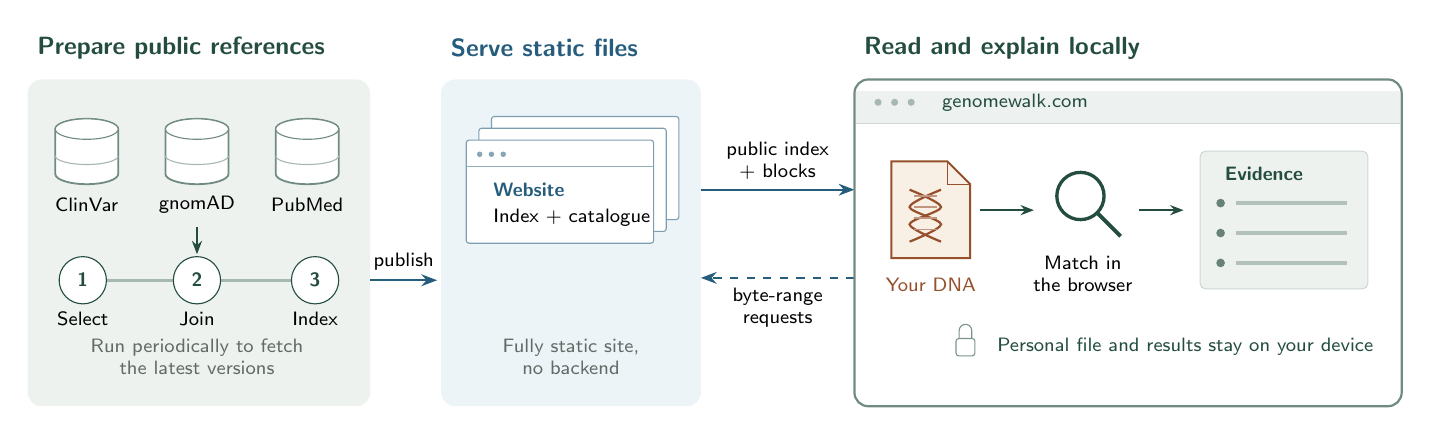
\begin{tikzpicture}[x=1cm,y=1cm,font=\sffamily\footnotesize,
  flow/.style={-{Stealth[length=2mm]},line width=.8pt,draw=inkblue},
  local/.style={-{Stealth[length=1.7mm]},line width=.8pt,draw=accent}]
% Three visual environments: a build pipeline, a file shelf, and a browser.
\node[anchor=west,font=\sffamily\bfseries\small,text=accent] at (0,4.35) {Prepare public references};
\node[anchor=west,font=\sffamily\bfseries\small,text=inkblue] at (5.25,4.35) {Serve static files};
\node[anchor=west,font=\sffamily\bfseries\small,text=accent] at (10.5,4.35) {Read and explain locally};
\fill[rounded corners=5pt,fill=tint] (0,-.20) rectangle (4.35,3.95);
\foreach \x/\name in {.75/ClinVar,2.15/gnomAD,3.55/PubMed} {
  \path[fill=white,draw=accent!65,line width=.65pt] (\x-.40,2.75) -- (\x-.40,3.32)
    arc[start angle=180,end angle=0,x radius=.40,y radius=.13] -- (\x+.40,2.75)
    arc[start angle=0,end angle=-180,x radius=.40,y radius=.13];
  \draw[accent!65,fill=white] (\x,3.32) ellipse (.40 and .13);
  \draw[accent!40] (\x-.40,2.98) arc[start angle=180,end angle=360,x radius=.40,y radius=.11];
  \node[font=\sffamily\scriptsize] at (\x,2.36) {\name};
}
\draw[local] (2.15,2.07)--(2.15,1.73);
\draw[accent!40,line width=1pt] (.70,1.40)--(3.65,1.40);
\foreach \x/\num/\label in {.70/1/Select,2.15/2/Join,3.65/3/Index} {
  \node[circle,draw=accent,fill=white,minimum size=6mm,inner sep=0pt,text=accent,font=\sffamily\bfseries\scriptsize] at (\x,1.40) {\num};
  \node[font=\sffamily\scriptsize] at (\x,.91) {\label};
}
\node[align=center,font=\sffamily\scriptsize,text=midgray] at (2.15,.43) {Run periodically to fetch\\the latest versions};
\draw[flow] (4.35,1.40)--node[above,font=\sffamily\scriptsize]{publish}(5.20,1.40);
% Static file cards, with no application-server or database icon.
\fill[rounded corners=5pt,fill=bluetint] (5.25,-.20) rectangle (8.55,3.95);
\foreach \x/\y in {5.89/2.17,5.73/2.02,5.57/1.87} {
  \path[fill=white,draw=inkblue!60,rounded corners=1pt] (\x,\y) rectangle +(2.38,1.31);
}
\draw[inkblue!50] (5.57,2.84)--(7.95,2.84);
\foreach \x in {5.74,5.89,6.04} {\fill[inkblue!55] (\x,3.00) circle (.035);}
\node[anchor=west,font=\sffamily\bfseries\scriptsize,text=inkblue] at (5.79,2.55) {Website};
\node[anchor=west,font=\sffamily\scriptsize] at (5.79,2.20) {Index + catalogue};
\node[align=center,font=\sffamily\scriptsize,text=midgray] at (6.90,.43) {Fully static site,\\no backend};
% Only public data cross the network boundary.
\draw[flow] (8.55,2.55)--node[above,align=center,font=\sffamily\scriptsize]{public index\\+ blocks}(10.50,2.55);
\draw[flow,dashed] (10.50,1.43)--node[below,align=center,font=\sffamily\scriptsize]{byte-range\\requests}(8.55,1.43);
% Browser chrome, local file, local matching, and a small result view.
\draw[draw=accent!65,fill=white,rounded corners=5pt,line width=.8pt] (10.50,-.20) rectangle (17.45,3.95);
\fill[accent!8] (10.52,3.40) rectangle (17.43,3.80);
\draw[linegray] (10.52,3.39)--(17.43,3.39);
\foreach \x in {10.80,11.01,11.22} {\fill[accent!40] (\x,3.66) circle (.045);}
\node[anchor=west,font=\sffamily\scriptsize,text=accent] at (11.49,3.65) {genomewalk.com};
\path[draw=copper,fill=warmtint,line width=.7pt] (10.97,1.68)--(10.97,2.91)--(11.68,2.91)--(11.97,2.62)--(11.97,1.68)--cycle;
\draw[copper] (11.68,2.91)--(11.68,2.62)--(11.97,2.62);
\draw[copper,line width=.8pt] plot[smooth] coordinates {(11.20,2.55)(11.60,2.33)(11.20,2.11)(11.60,1.89)};
\draw[copper,line width=.8pt] plot[smooth] coordinates {(11.60,2.55)(11.20,2.33)(11.60,2.11)(11.20,1.89)};
\foreach \y in {2.47,2.33,2.19,2.05} {\draw[copper!60] (11.26,\y)--(11.55,\y);}
\node[font=\sffamily\scriptsize,text=copper] at (11.47,1.34) {Your DNA};
\draw[local] (12.10,2.29)--(12.78,2.29);
\draw[accent,line width=1.2pt] (13.37,2.47) circle (.30);
\draw[accent,line width=1.4pt] (13.59,2.25)--(13.88,1.96);
\node[align=center,font=\sffamily\scriptsize] at (13.40,1.48) {Match in\\the browser};
\draw[local] (14.12,2.29)--(14.68,2.29);
\draw[linegray,fill=tint,rounded corners=2pt] (14.89,1.29) rectangle (17.02,3.04);
\node[anchor=west,font=\sffamily\bfseries\scriptsize,text=accent] at (15.08,2.75) {Evidence};
\foreach \y in {2.38,2.00,1.62} {
  \fill[accent!70] (15.15,\y) circle (.055);
  \draw[accent!35,line width=1.5pt] (15.35,\y)--(16.75,\y);
}
\draw[accent!60,rounded corners=1pt] (11.79,.44) rectangle (12.03,.66);
\draw[accent!60] (11.83,.66)--(11.83,.76) arc[start angle=180,end angle=0,radius=.08]--(11.99,.66);
\node[anchor=west,font=\sffamily\scriptsize,text=accent] at (12.19,.56) {Personal file and results stay on your device};
\end{tikzpicture}
\caption{Public references travel to the browser; personal genome processing stays on the device. The website needs only static files. Requested catalogue ranges remain visible to the host.}
\label{fig:architecture}
\end{figure*}

The browser reads VCF files and DNA files from services such as 23andMe and AncestryDNA. The guide explains the information available in each file. Large VCFs are read in small chunks instead of being loaded all at once. Supported compressed files from these services are unpacked in the browser, with size limits to control memory use.

\section{Offline reference preparation}
The offline job turns public data into compact reference files for the website. Table~\ref{tab:data-sources} lists the sources and their roles. It produces a catalogue and lookup index for each supported reference genome (GRCh38 and GRCh37), plus separate teaching examples. These reference genomes are two versions of the map used to give variants their addresses.

\par\smallskip\noindent
\begin{minipage}{\columnwidth}
\small
\captionsetup{type=table}
\caption{Public data sources used in reference preparation.}
\label{tab:data-sources}
\begin{tabularx}{\linewidth}{@{}>{\raggedright\arraybackslash}p{0.23\linewidth}>{\raggedright\arraybackslash}X@{}}
\toprule
\textbf{Data source} & \textbf{What we use it for} \\
\midrule
ClinVar~\cite{clinvar} & Variant identities, classifications, review stars, genes, conditions and links to cited publications. \\
\addlinespace
gnomAD~\cite{gnomad} & Population frequencies for catalogue variants and ancestry-group frequencies for teaching examples. \\
\addlinespace
PubMed~\cite{pubmed} & Author, journal and year for readable publication labels. \\
\bottomrule
\end{tabularx}
\end{minipage}
\par\smallskip

Build scripts read gnomAD's published combined-frequency files using a standard Tabix reader~\cite{tabixjs}. Their indexes locate the relevant regions, so the offline job can request parts of these large files. Completed regions are cached for reuse.

\subsection{From public records to a ready-to-use catalogue}
The offline job uses public reference data only; it does not use anyone's personal DNA file.

\subsubsection*{1. Choose which records to include}
Genomewalk keeps ClinVar entries labelled pathogenic, likely pathogenic, conflicting, drug response, risk, association, protective or related categories. Entries labelled benign, likely benign or uncertain significance are left out. This defines the guide's scope; it is not a comprehensive clinical screen. See Figure~\ref{fig:offline-build} for examples of which rows are included or omitted and why.

Each row must describe one alternative DNA sequence. The reference sequence (\code{REF}) and alternative (\code{ALT}) must each contain at most 50 letters: A, C, G, T or N, where N marks an unspecified base. For example, \code{C} to \code{T} and \code{A} to \code{AT} can be kept. An ALT of \code{A,G} lists two alternatives, while \code{<DEL>} names a deletion without spelling out its sequence; both are omitted.

\begin{figure*}[t]
\centering
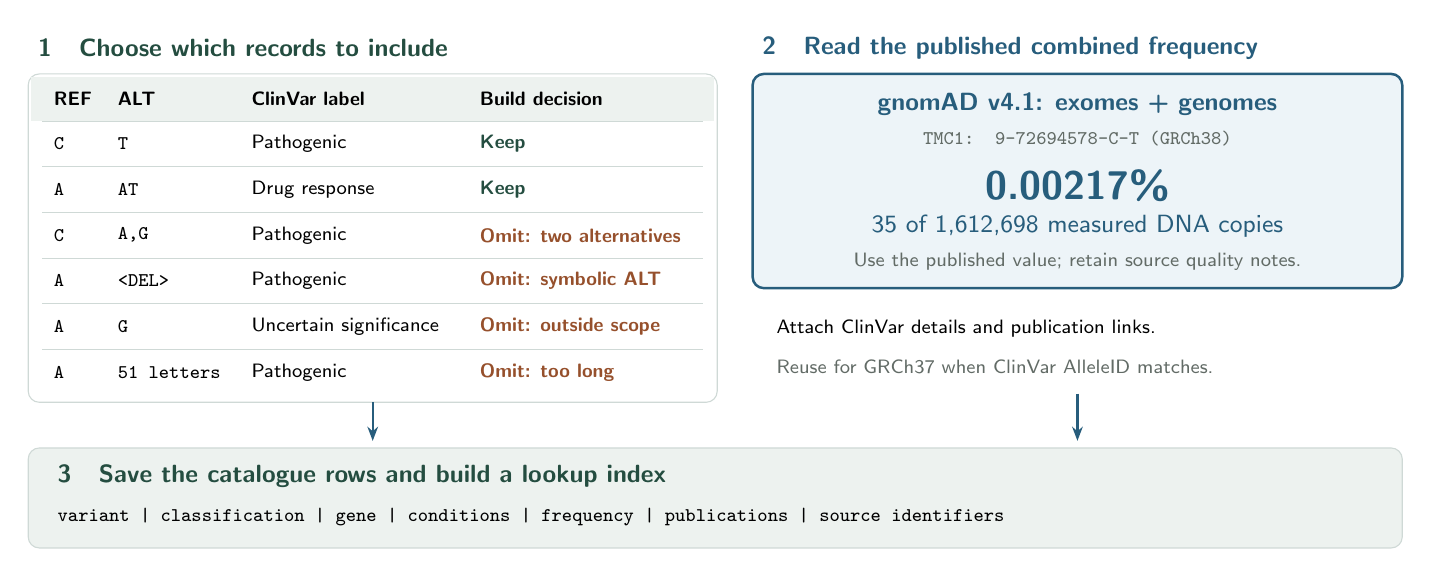
\begin{tikzpicture}[x=1cm,y=1cm,font=\sffamily\footnotesize,
  flow/.style={-{Stealth[length=1.8mm]},line width=.8pt,draw=inkblue}]
\node[anchor=west,font=\sffamily\bfseries\small,text=accent] at (0,6.35) {1\quad Choose which records to include};
\node[anchor=west,font=\sffamily\bfseries\small,text=inkblue] at (9.20,6.35) {2\quad Read the published combined frequency};
% The table shows both the classification filter and the sequence-format filter.
\draw[linegray,fill=white,rounded corners=4pt] (0,1.85) rectangle (8.75,6.02);
\fill[tint] (.04,5.42) rectangle (8.71,5.98);
\node[anchor=west,inner sep=0pt,font=\sffamily\bfseries\scriptsize] at (.32,5.70) {REF};
\node[anchor=west,inner sep=0pt,font=\sffamily\bfseries\scriptsize] at (1.13,5.70) {ALT};
\node[anchor=west,inner sep=0pt,font=\sffamily\bfseries\scriptsize] at (2.83,5.70) {ClinVar label};
\node[anchor=west,inner sep=0pt,font=\sffamily\bfseries\scriptsize] at (5.73,5.70) {Build decision};
\foreach \y in {5.42,4.84,4.26,3.68,3.10,2.52} {\draw[linegray] (.18,\y)--(8.57,\y);}
\foreach \y/\refbase/\altbase/\classification/\decision/\tone in {
5.13/C/T/Pathogenic/Keep/accent,
4.55/A/AT/Drug response/Keep/accent,
3.97/C/{A,G}/Pathogenic/{Omit: two alternatives}/copper,
3.39/A/{<DEL>}/Pathogenic/{Omit: symbolic ALT}/copper,
2.81/A/G/{Uncertain significance}/{Omit: outside scope}/copper,
2.23/A/{51 letters}/Pathogenic/{Omit: too long}/copper} {
  \node[anchor=west,inner sep=0pt,font=\ttfamily\scriptsize] at (.32,\y) {\refbase};
  \node[anchor=west,inner sep=0pt,font=\ttfamily\scriptsize] at (1.13,\y) {\altbase};
  \node[anchor=west,inner sep=0pt,font=\sffamily\scriptsize] at (2.83,\y) {\classification};
  \node[anchor=west,inner sep=0pt,font=\sffamily\bfseries\scriptsize,text=\tone] at (5.73,\y) {\decision};
}
% Real published joint gnomAD entry, not a locally averaged estimate.
\draw[inkblue,line width=.9pt,fill=bluetint,rounded corners=4pt] (9.20,3.30) rectangle (17.45,6.02);
\node[font=\sffamily\bfseries\small,text=inkblue] at (13.325,5.64) {gnomAD v4.1: exomes + genomes};
\node[font=\ttfamily\scriptsize,text=midgray] at (13.325,5.20) {TMC1: 9-72694578-C-T (GRCh38)};
\node[font=\sffamily\bfseries\Large,text=inkblue] at (13.325,4.60) {0.00217\%};
\node[font=\sffamily\small,text=inkblue] at (13.325,4.09) {35 of 1,612,698 measured DNA copies};
\node[font=\sffamily\scriptsize,text=midgray] at (13.325,3.63) {Use the published value; retain source quality notes.};
\node[anchor=west,font=\sffamily\scriptsize] at (9.38,2.78) {Attach ClinVar details and publication links.};
\node[anchor=west,font=\sffamily\scriptsize,text=midgray] at (9.38,2.30) {Reuse for GRCh37 when ClinVar AlleleID matches.};
% The output is one enriched row, followed by the index used in the next figure.
\draw[flow] (4.375,1.85)--(4.375,1.36);
\draw[flow] (13.325,1.96)--(13.325,1.36);
\draw[linegray,fill=tint,rounded corners=4pt] (0,0) rectangle (17.45,1.27);
\node[anchor=west,font=\sffamily\bfseries\small,text=accent] at (.25,.91) {3\quad Save the catalogue rows and build a lookup index};
\node[anchor=west,font=\ttfamily\scriptsize] at (.25,.39) {variant | classification | gene | conditions | frequency | publications | source identifiers};
\end{tikzpicture}
\caption{Building the public catalogue. Simplified, hypothetical rows show the selection rules. The real TMC1 frequency comes from gnomAD's joint release. The counts describe DNA copies, not people; the displayed percentage is rounded. The output row shows a subset of the saved fields.}
\label{fig:offline-build}
\end{figure*}

\subsubsection*{2. Add the evidence}
Kept rows retain ClinVar's classification, review status, conditions and source identifiers. If ClinVar lists several genes, the current build stores the first listed name only; it does not rank which gene matters most. Condition names link to MedGen, NCBI's directory of medical conditions, using identifiers already supplied by ClinVar~\cite{medgen}. When names and identifiers cannot be paired reliably, the name remains without that direct link. Publication IDs are attached using the ClinVar record number (VariationID); PubMed supplies readable citation labels. A reference can be a general methods paper or guideline, rather than a study showing that this variant causes a condition.

gnomAD v4.1 publishes combined frequencies from exome and whole-genome studies~\cite{gnomad}. Exomes cover mainly protein-making DNA; genome studies read more broadly. Genomewalk imports the published frequencies and counts rather than choosing a dataset or averaging percentages. Figure~\ref{fig:offline-build} shows a real example: 35 TMC1 variant copies among 1,612,698 measured copies. Results retain cautions about failed source quality filters and disagreement between datasets (gnomAD's threshold: $p<0.0001$). Missing values remain unknown.

The same variant can have different addresses in GRCh37 and GRCh38. The build first finds its gnomAD frequency using the GRCh38 address. It then reuses that frequency for a GRCh37 entry only when ClinVar gives both entries the same variant identifier (AlleleID)~\cite{clinvarids}. Both catalogues therefore use the same v4.1 frequency and quality information. The original gnomAD address is saved so the source can be checked. This links records for the same variant; it does not convert the user's file between genome versions.

\subsubsection*{3. Check and publish the files}
The job writes annotated rows to a compressed catalogue and builds an index locating each row (Section~\ref{sec:retrieval}). Teaching examples use the same combined-frequency source, with curated variant addresses for each build. Periodic runs can reuse complete cached inputs or fetch updated sources. Outputs include source dates and identifiers, are validated, and replace previous files only after successful generation. Each catalogue must be published with its matching index. Reproducing an output requires the same inputs, tool versions and build rules.

\section{Selective catalogue retrieval}
\label{sec:retrieval}
The browser needs annotations for matched variants, not every entry in the catalogue. A small index tells it where those annotations are stored. The catalogue uses BGZF: a gzip-compatible format made of blocks that can be decompressed independently~\cite{bgzf}. HTTP byte-range requests retrieve selected blocks from the static file~\cite{http}.

\subsection{From a variant to a catalogue row}
The browser downloads a compressed JSON index and decompresses it locally. Its JSON has two lookup lists: \code{records} links variant keys to rows; \code{blocks} gives the byte location and size of each compressed block. A key combines chromosome, position, reference allele and alternate allele, within the specified genome build.

Figure~\ref{fig:range} follows one hypothetical input through real index entries. The key \code{1:1232816:C:T} selects block 1. That block starts at byte 11,138 and occupies 11,670 compressed bytes, so the request ends at byte 22,807. Once checked and decompressed, it contains 65,280 bytes. The matched row starts at offset 118 and occupies 419 bytes. This example uses an earlier catalogue snapshot; rebuilding the catalogue changes its offsets and hashes. Section~\ref{sec:evaluation} reports a separate benchmark snapshot.

\begin{figure*}[t]
\centering
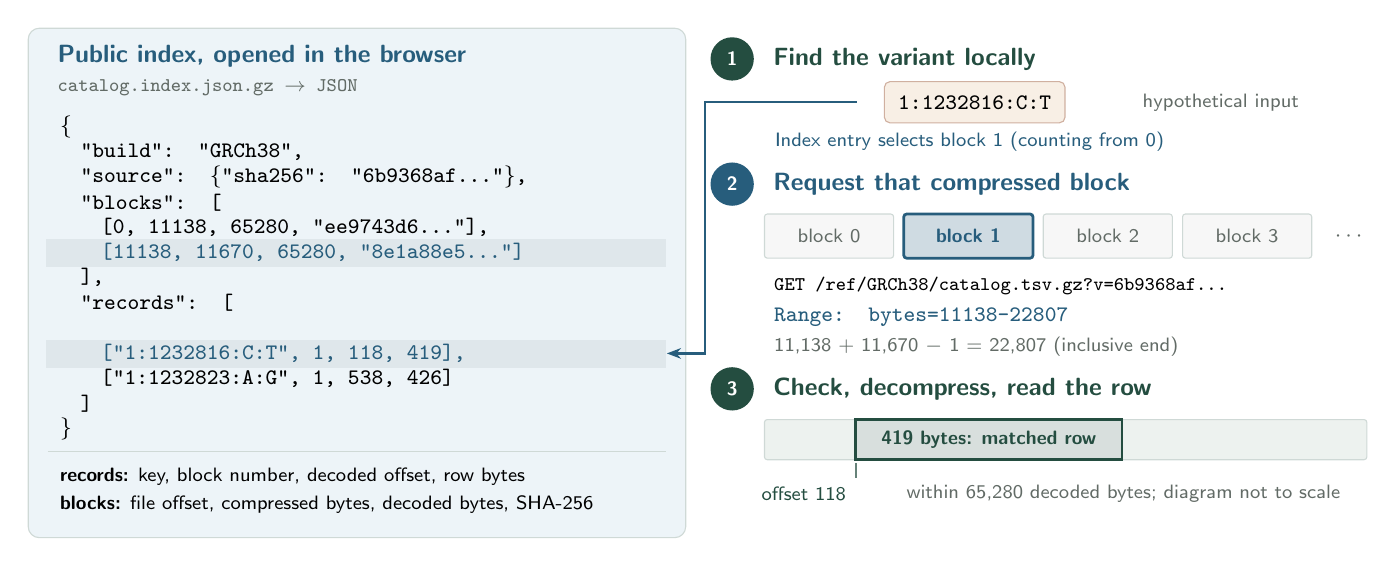
\begin{tikzpicture}[x=1cm,y=1cm,font=\sffamily\footnotesize,
  flow/.style={-{Stealth[length=1.8mm]},line width=.8pt,draw=inkblue}]
% A real, shortened JSON excerpt. Blue links the selected record to block 1.
\draw[linegray,fill=bluetint,rounded corners=4pt] (0,0) rectangle (8.35,6.47);
\node[anchor=west,font=\sffamily\bfseries\small,text=inkblue] at (.25,6.11) {Public index, opened in the browser};
\node[anchor=west,font=\ttfamily\scriptsize,text=midgray] at (.25,5.72) {catalog.index.json.gz $\rightarrow$ JSON};
\fill[inkblue!15] (.22,3.44) rectangle (8.10,3.79);
\fill[inkblue!15] (.22,2.16) rectangle (8.10,2.51);
\node[anchor=west,font=\ttfamily\footnotesize] at (.28,5.22) {\{};
\node[anchor=west,font=\ttfamily\footnotesize] at (.54,4.90) {"build": "GRCh38",};
\node[anchor=west,font=\ttfamily\footnotesize] at (.54,4.58) {"source": \{"sha256": "6b9368af..."\},};
\node[anchor=west,font=\ttfamily\footnotesize] at (.54,4.26) {"blocks": [};
\node[anchor=west,font=\ttfamily\footnotesize] at (.80,3.94) {[0, 11138, 65280, "ee9743d6..."],};
\node[anchor=west,font=\ttfamily\footnotesize\bfseries,text=inkblue] at (.80,3.62) {[11138, 11670, 65280, "8e1a88e5..."]};
\node[anchor=west,font=\ttfamily\footnotesize] at (.54,3.30) {],};
\node[anchor=west,font=\ttfamily\footnotesize] at (.54,2.98) {"records": [};
\node[anchor=west,font=\ttfamily\footnotesize\bfseries,text=inkblue] at (.80,2.34) {["1:1232816:C:T", 1, 118, 419],};
\node[anchor=west,font=\ttfamily\footnotesize] at (.80,2.02) {["1:1232823:A:G", 1, 538, 426]};
\node[anchor=west,font=\ttfamily\footnotesize] at (.54,1.70) {]};
\node[anchor=west,font=\ttfamily\footnotesize] at (.28,1.38) {\}};
\draw[linegray] (.25,1.10)--(8.10,1.10);
\node[anchor=west,font=\sffamily\scriptsize] at (.28,.78) {\textbf{records:} key, block number, decoded offset, row bytes};
\node[anchor=west,font=\sffamily\scriptsize] at (.28,.42) {\textbf{blocks:} file offset, compressed bytes, decoded bytes, SHA-256};
% A browser-local lookup and the corresponding public-file request.
\node[circle,fill=accent,text=white,inner sep=0pt,minimum size=5.5mm,font=\sffamily\bfseries\scriptsize] at (8.94,6.08) {1};
\node[anchor=west,font=\sffamily\bfseries\small,text=accent] at (9.34,6.08) {Find the variant locally};
\node[draw=copper!45,fill=warmtint,rounded corners=2pt,inner sep=5pt,font=\ttfamily\footnotesize] at (12.02,5.53) {1:1232816:C:T};
\node[anchor=west,font=\sffamily\scriptsize,text=midgray] at (14.03,5.53) {hypothetical input};
\draw[flow] (10.52,5.53)--(8.59,5.53)--(8.59,2.34)--(8.11,2.34);
\node[anchor=west,font=\sffamily\scriptsize,text=inkblue] at (9.36,5.03) {Index entry selects block 1 (counting from 0)};
\node[circle,fill=inkblue,text=white,inner sep=0pt,minimum size=5.5mm,font=\sffamily\bfseries\scriptsize] at (8.94,4.49) {2};
\node[anchor=west,font=\sffamily\bfseries\small,text=inkblue] at (9.34,4.49) {Request that compressed block};
\foreach \x/\label in {9.35/0,11.12/1,12.89/2,14.66/3} {
  \draw[draw=linegray,fill=black!3,rounded corners=1pt] (\x,3.55) rectangle +(1.64,.56);
  \node[font=\sffamily\scriptsize,text=midgray] at (\x+.82,3.83) {block \label};
}
\draw[draw=inkblue,fill=inkblue!22,line width=1pt,rounded corners=1pt] (11.12,3.55) rectangle +(1.64,.56);
\node[font=\sffamily\bfseries\scriptsize,text=inkblue] at (11.94,3.83) {block 1};
\node[text=midgray] at (16.77,3.83) {$\cdots$};
\node[anchor=west,font=\ttfamily\scriptsize] at (9.35,3.20) {GET /ref/GRCh38/catalog.tsv.gz?v=6b9368af...};
\node[anchor=west,font=\ttfamily\footnotesize\bfseries,text=inkblue] at (9.35,2.80) {Range: bytes=11138-22807};
\node[anchor=west,font=\sffamily\scriptsize,text=midgray] at (9.35,2.42) {11,138 + 11,670 $-$ 1 = 22,807 (inclusive end)};
\node[circle,fill=accent,text=white,inner sep=0pt,minimum size=5.5mm,font=\sffamily\bfseries\scriptsize] at (8.94,1.89) {3};
\node[anchor=west,font=\sffamily\bfseries\small,text=accent] at (9.34,1.89) {Check, decompress, read the row};
\draw[draw=linegray,fill=tint,rounded corners=1pt] (9.35,.99) rectangle (17.00,1.50);
\draw[draw=accent,fill=accent!18,line width=1pt] (10.51,.99) rectangle (13.89,1.50);
\node[font=\sffamily\bfseries\scriptsize,text=accent] at (12.20,1.25) {419 bytes: matched row};
\draw[accent!70,line width=.7pt] (10.51,.95)--(10.51,.76);
\node[anchor=east,font=\sffamily\scriptsize,text=accent] at (10.51,.56) {offset 118};
\node[anchor=west,font=\sffamily\scriptsize,text=midgray] at (11.03,.56) {within 65,280 decoded bytes; diagram not to scale};
\end{tikzpicture}
\caption{One variant, one catalogue block. The hypothetical input is matched against real GRCh38 index entries. The JSON is an excerpt: other entries and fields are omitted, and hashes are shortened. After decompression, the browser reads bytes 118--536 of the block (419 bytes). Neighbouring rows arrive too; no personal variant key is sent in the request.}
\label{fig:range}
\end{figure*}

The request's \code{v=} value comes from the catalogue hash in the index; it distinguishes releases in caches. Full SHA-256 hashes are used in requests and validation. The figure shortens them only for readability.

Several matches can share a block. The browser downloads each required block once per lookup, combines adjacent selected blocks into one request, and runs up to four requests at a time. A row spanning blocks requires each one. Decoded annotations are reused during the visit.

Before displaying an annotation, the browser checks the \code{206 Partial Content} response, byte range and length, each block's hash and decoded size, and the reconstructed variant key. A full-file \code{200} response or changed encoding stops the lookup with an error. The host must preserve the compressed file's bytes.

\subsection{What is downloaded}
For an uncached lookup, catalogue traffic is the compressed index plus the selected compressed blocks. Many matches, or matches spread across the file, can reduce the savings. Extra requests can also add delay, so fewer bytes do not guarantee a faster result.

Small teaching-example and consumer lookup files are downloaded whole. Reading and matching a personal genome still requires scanning the local file. The optional public HG002 sample is different: its bytes are downloaded in chunks because that sample is hosted online.

\section{Matching rules and supported files}
A match requires the same genome build, chromosome, position, reference allele and alternate allele. Genomewalk supports GRCh37 and GRCh38 but does not convert coordinates between them. It recognises chromosome-name aliases, such as \code{chr1} and \code{1}.

\textbf{Identifying the reference build.} Genomewalk checks reference names, assembly labels and declared chromosome lengths in VCF headers, and build names in consumer-file comments. It recognises common aliases, including hg19 and hg38. For AncestryDNA exports without build information, it uses the documented GRCh37 format. If the build remains unknown, the reader is asked to choose GRCh37, GRCh38 or ``Another build / I'm not sure'' before matching. Manual choices are labelled ``Selected by you'' and apply only to that file for the current visit. Unresolved builds, conflicting metadata and recognised unsupported builds allow file exploration without catalogue matching.

\textbf{Sequencing files (VCF).} The browser reads the first sample in a BGZF VCF/gVCF and checks for damaged or incomplete blocks. A result must contain an alternate allele reported in the sample, with \code{FILTER=PASS} or \code{.}. The dot means no filter was declared; it does not certify call quality. Incomplete calls retain warnings. Duplicate variant keys are merged, with contradictory calls flagged.

Insertions and deletions must have the same written representation as the catalogue entry. For example, \code{T}$\rightarrow$\code{TC} can match at the same build and coordinate. An equivalent change written differently can be missed because the application does not standardise indel representations.

\textbf{Consumer exports.} Supported 23andMe and AncestryDNA files are checked for provider, genome build and strand. Matching accepts complete, two-allele A/C/G/T single-base calls on autosomes (chromosomes 1--22). Known rsIDs are cross-checked against coordinates. Conflicting duplicates, missing calls, sex-chromosome calls and insertion/deletion codes such as \code{I/D} are excluded from interpretation. These codes do not specify the changed sequence. ZIP/gzip imports allow one text payload, at most 128\,MiB unpacked and two million rows.

\section{Privacy and its limits}
Genomewalk reads the selected personal file locally. It does not upload the filename, genomic contents or results, and uses no remote matching service or language model to analyse the genome. File handles and results stay in memory for the visit; refreshing requires selecting the file again. This does not guarantee secure erasure from the browser or operating system.

Local processing does not hide every clue about the analysis. The host sees IP addresses, timing and requested public-file ranges. Because those ranges correspond to known catalogue records, they can suggest which variants matched. Clicking a source link also tells that provider which public record was opened. Font requests and hosting analytics expose additional connection or usage metadata; the application does not add genomic contents or results to analytics.

HTTPS protects data in transit. Hash checks detect corrupted blocks or mixed catalogue releases, but cannot protect against a publisher replacing both the application and its index. The design therefore assumes a trusted browser, device and application. It has not undergone an independent security audit. Public assets still need network access unless already available locally.

\section{Learning from the file and the evidence}
The guide starts with the file: its header, a variant row, variant types and summary counts. It then introduces gnomAD frequencies, ClinVar classifications and the user's matches. Readers can explore in any order or go straight to results.

Examples from the file show why records are included or omitted. The interface distinguishes file rows from genomic sites, possible alleles from the reported genotype, and unsupported records from missing evidence. Curated teaching examples remain separate from personal results. Result categories separate disease evidence, drug response, traits and associations.

Each annotation answers a different question. Genotype and quality describe the file. ClinVar classification describes a submitted claim; review stars describe how that classification was reviewed, not whether the user's genotype is correct~\cite{review}. Population frequency describes sampled allele copies, not personal risk, and missing frequency is not shown as zero. Source links let readers inspect the evidence. A catalogue match alone neither diagnoses nor rules out a condition.

\section{Preliminary engineering evaluation}
\label{sec:evaluation}
\subsection{Catalogue download comparison}
We compared full-catalogue and selective downloads using the public NIST Genome in a Bottle HG002 GRCh38 v5.0q sample~\cite{hg002}. Both paths produced 399 identical result objects, including their annotations. Table~\ref{tab:transfer} counts a complete compressed catalogue for the baseline, versus the compressed index and requested blocks for the selective path. Neither starts with cached reference files.

\begin{table}[t]
\caption{Catalogue payload for HG002. Figures exclude the sample, application assets, other reference files and HTTP overhead.}
\label{tab:transfer}
\centering\small
\begin{tabularx}{\columnwidth}{@{}Xr@{}}
\toprule
\textbf{Component} & \textbf{Bytes}\\
\midrule
Complete catalogue (baseline) & 26,640,645\\
Index (selective path) & 5,154,640\\
Annotation blocks, 203 requests & 2,745,473\\
\textbf{Total selective payload} & \textbf{7,900,113}\\
\bottomrule
\end{tabularx}
\end{table}

The selective path used 70.3\% fewer catalogue bytes while preserving the results for this sample. This comparison does not measure overall speed. Request delays, match density, caching and network conditions also affect the time a user waits.

\subsection{Reference snapshot and software checks}
The earlier benchmark snapshot predates the combined-frequency importer. Its GRCh38 catalogue contains 511,197 records in 2,524 blocks; GRCh37 contains 511,193 records in 2,457 blocks. Compressed sizes are 26.64 and 25.49\,MB respectively, with approximately 5.15\,MB indexes (decimal units). The companion engineering snapshot retains exact sizes and hashes.

That benchmark version passed 182 tests, along with type, lint, build and deployment checks. Tests cover file reading, invalid inputs, matching rules, reference consistency, byte-range reconstruction and cancellation. They check software behaviour, not clinical sensitivity or comprehensive security. The HG002 comparison checks that both retrieval paths give the same output; it does not assess the accuracy of the sample's variant calls.

\section{Discussion and limitations}
Selective downloads reduce bandwidth but expose which public catalogue regions were requested. Downloading the full catalogue could reduce that signal at a higher transfer cost; concealing queries more fully would require a different design.

Coverage is limited by the selected catalogue and matching rules. Genomewalk does not infer missing genotypes, ancestry, polygenic risk or parental origin, and it does not make diagnoses. Supporting equivalent indel representations or consumer insertion/deletion codes would require further validated handling of builds, strands and file formats.

Evaluation is preliminary and developer-conducted. One public sample does not establish performance across files, browsers or devices. There is no user-comprehension study, independent security audit or clinical validation. A useful next study would ask whether readers better understand exclusions, catalogue matches and the difference between population frequency and personal risk. Broader engineering tests should measure memory use, responsiveness, download sizes and waiting times.

\section{Conclusion}
Genomewalk combines local genome processing, prepared public references and selective downloads with a guide to understanding the evidence. The public-sample comparison preserved results while reducing catalogue traffic. The next step is to test how well the explanations help readers and how the software performs across a wider range of inputs.

\section*{Artifact availability}
The accompanying source tree contains the application, reference builders and technical documentation. Code is MIT-licensed; public datasets retain their own terms. The draft's engineering snapshot records the benchmark inputs and outputs. A fixed public release and a reusable benchmark runner should accompany publication. No private genomic file was used in the reported comparison.

\balance
\begin{thebibliography}{10}
\small
\setlength{\itemsep}{3pt}
\setlength{\parskip}{0pt}
\bibitem{promethease} Promethease. \emph{Service overview and privacy policy}. \url{https://promethease.com/}; \url{https://promethease.com/privacy}.
\bibitem{biocodify} Biocodify. \emph{Product overview and privacy policy}. \url{https://biocodify.com/}; \url{https://biocodify.com/privacy}.
\bibitem{deana} DeanaDNA. \emph{Deana: project documentation and privacy model}. \url{https://github.com/DeanaDNA/deana}.
\bibitem{allelix} Allelix. \emph{Genotype analysis toolkit: project documentation}. \url{https://github.com/allelix/allelix}.
\bibitem{interpretome} K.~J. Karczewski et al. Interpretome: a freely available, modular, and secure personal genome interpretation engine. \emph{Pacific Symposium on Biocomputing}, 17:339--350, 2012. \url{https://psb.stanford.edu/psb-online/proceedings/psb12/karczewski.pdf}.
\bibitem{myseq} M.~D. Linderman, L. McElroy, and L. Chang. MySeq: privacy-protecting browser-based personal genome analysis for genomics education and exploration. \emph{BMC Medical Genomics}, 12:172, 2019. \doi{10.1186/s12920-019-0615-3}.
\bibitem{igv} J.~T. Robinson, H. Thorvaldsd\'{o}ttir, D. Turner, and J.~P. Mesirov. igv.js: an embeddable JavaScript implementation of the Integrative Genomics Viewer (IGV). \emph{Bioinformatics}, 39(1):btac830, 2023. \doi{10.1093/bioinformatics/btac830}.
\bibitem{igvweb} IGV Team. \emph{IGV-Web App documentation}. \url{https://igv.org/doc/webapp/}. Accessed September 2026.
\bibitem{fileapi} World Wide Web Consortium. \emph{File API}. \url{https://www.w3.org/TR/FileAPI/}. Accessed September 2026.
\bibitem{clinvar} NCBI. \emph{ClinVar: Introduction}. \url{https://www.ncbi.nlm.nih.gov/clinvar/intro/}. Accessed September 2026.
\bibitem{gnomad} gnomAD Production Team. \emph{gnomAD v4.1}, April 2024. \url{https://gnomad.broadinstitute.org/news/2024-04-gnomad-v4-1}.
\bibitem{pubmed} NCBI. \emph{Get article metadata: PubMed E-Summary}. \url{https://pmc.ncbi.nlm.nih.gov/tools/get-metadata/}.
\bibitem{tabixjs} GMOD. \emph{Tabix indexed-file reader for JavaScript}. \url{https://github.com/GMOD/tabix-js}.
\bibitem{medgen} NCBI. \emph{MedGen overview}. \url{https://www.ncbi.nlm.nih.gov/medgen/docs/overview/}.
\bibitem{clinvarids} NCBI. \emph{Identifiers in ClinVar}. \url{https://www.ncbi.nlm.nih.gov/clinvar/docs/identifiers/}.
\bibitem{bgzf} HTSlib / SAMtools. \emph{bgzip manual}. \url{https://www.htslib.org/doc/bgzip.html}. Accessed September 2026.
\bibitem{http} R. Fielding, M. Nottingham, and J. Reschke, eds. \emph{HTTP Semantics}. RFC 9110, June 2022, sections 14 and 15.3.7. \doi{10.17487/RFC9110}.
\bibitem{review} NCBI. \emph{Review status in ClinVar}. \url{https://www.ncbi.nlm.nih.gov/clinvar/docs/review_status/}. Accessed September 2026.
\bibitem{hg002} NIST / Genome in a Bottle Consortium. \emph{HG002 GRCh38 v5.0q small-variant release}. \href{https://ftp-trace.ncbi.nlm.nih.gov/ReferenceSamples/giab/release/AshkenazimTrio/HG002_NA24385_son/v5.0q/}{Public release directory}. Release files, checksums and terms.
\end{thebibliography}
\end{document}
